\chapter{Results}
In the attack, a personalized Bash script (ddos.sh) was initiated and distributed among bot computers. Both scripts used the hping3 utility to create high rates of UDP packets thrown at the target (192.168.56.101). The attack itself was controlled by the main attacking computer (192.168.0.59) and it communicated with the bots over SSH.
\section{Victim machine status before the attack}
\begin{figure}[!htb]
    \centering
    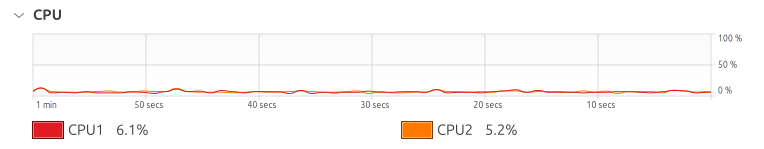
\includegraphics[width=0.8\linewidth]{thesis/cpuBefore.png}
    \caption{CPU usage before the attack}
    \label{fig:enter-label}
\end{figure}
\begin{figure}[!htb]
    \centering
    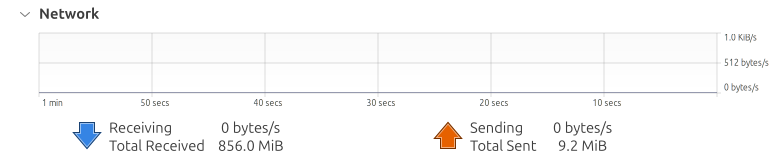
\includegraphics[width=0.8\linewidth]{thesis/beforeAttack.png}
    \caption{Traffic through the server before the attack}
    \label{fig:enter-label}
\end{figure}
\section{Victim machine status during the attack}
\\Run the script start\_attack.sh.
\begin{figure}[!htb]
    \centering
    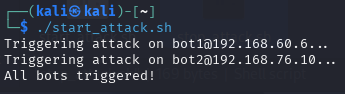
\includegraphics[width=0.5\linewidth]{thesis/startAttack.png}
    \caption{Execute start\_attack.sh}
    \label{fig:enter-label}
\end{figure}
\\ After executing the script, the victim machine experiences a noticeable spike in traffics and resource usage. This project showcases four different scenarios with different settings to see the effectiveness of Suricata in each case.
\\
\subsection{Scenario 1: UDP Flood Attack without Suricata}
\\We will first use the hping3 flood command to conduct a udp flood attack.
\begin{lstlisting}[language=bash,caption={Content of ddos.sh}]
$ sudo hping3 -d 65495 --udp --flood 192.168.56.101
\end{lstlisting}
\\During this scenario, we can observe that the victim experiences a huge spike in bandwidth and cpu usage.
\\
\begin{figure}[!htb]
    \centering
    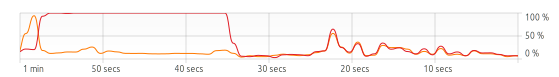
\includegraphics[width=0.8\linewidth]{thesis/cpuAfter.png}
    \caption{CPU usage during the flood attack (without Suricata)}
    \label{fig:enter-label}
\end{figure}
\begin{figure}[!htb]
    \centering
    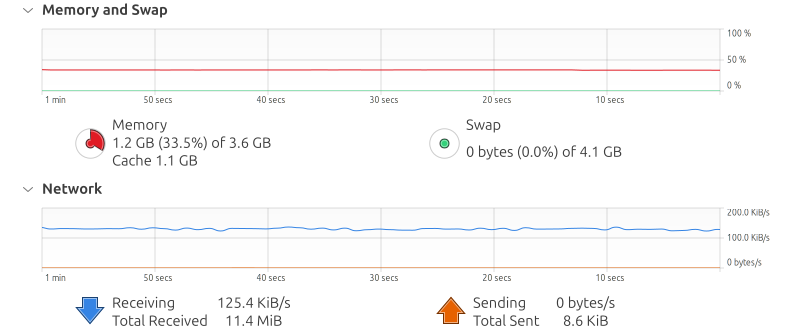
\includegraphics[width=0.8\linewidth]{thesis/afterAttack.png}
    \caption{Traffic through the server during the flood attack (without Suricata)}
    \label{fig:enter-label}
\end{figure}
\\
During the DDoS simulation, Wireshark's IPv4 Statistics \– All Addresses tool was used to analyze packet distribution across the network. A total of 48,082 IPv4 packets were captured. The majority of these packets were either sent by the attacker or received by the target server, indicating a high-volume flood behavior consistent with a UDP-based DDoS attack. The following are the statistic table and an image capture from Wireshark.
\begin{table}[!htb]
    \centering
    \scalebox{0.8}{
    \begin{tabular}{|m{6em}|c|c|c|c|c|c|c|c|}
    \hline
      Topic/Item & Count & Average & Min Val & Max Val & Rate(ms) & Percent & Burst Rate & Burst Start \\ 
      \hline
      IPv4 Statsistics/All addresses & 48082 &  &  & & 0.0874 & 100\% & 0.1100 & 19.685 \\
      \hline
      224.0.0.251 & 1 & & & & 0.0000 & 0.00\% & 0.0100 & 254.699 \\
      \hline
      192.168.76.10 & 20167 & & & & 0.0367 & 41.94\% & 0.1100 & 228.066 \\
      \hline
      192.168.60.6 & 27914 & & & & 0.0507 & 58.05\% & 0.1100 & 19.685 \\
      \hline
      192.168.56.101 & 48082 & & & & 0.0874 & 100.00\% & 0.1100 & 19.685\\
      \hline
    \end{tabular}}
    \caption{Wireshark statistics after attack}
    \label{tab:my_label}
\end{table}
\\
\begin{figure}[!htb]
    \centering
    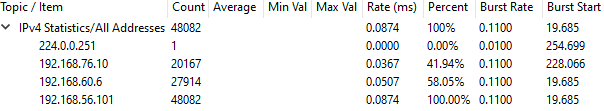
\includegraphics[width=0.8\linewidth]{thesis/wiresharkCapture1.png}
    \caption{IPv4 Statistics after the attack}
    \label{fig:enter-label}
\end{figure}
\\
The primary victim machine (192.168.56.101) received all 48,082 packets (100\% of traffic), confirming its role as the target of the attack. The main attacker bot (192.168.60.6) was responsible for 27,914 packets, accounting for 58.05\% of the total packet traffic. A secondary node (192.168.76.10) generated 20,167 packets, contributing 41.94\% of the traffic. This distribution suggests the involvement of multiple bots in generating the flood, which mirrors a typical distributed denial-of-service attack scenario.

A single multicast packet was recorded, sent to 224.0.0.251, a standard mDNS address, and was not related to attack traffic \cite{cirani2018internet}. The burst rate for both the attacking IP and the victim peaked at 0.1100 ms, with the burst start time at 19.685s, pinpointing the initiation of the attack in the traffic timeline. The attack packets were transmitted at high speed, with inter-packet rates of 0.0367 ms and 0.0507 ms for the attackers, reflecting sustained and aggressive traffic delivery.
\\
\subsection{Scenario 2: UDP Flood Attack with Suricata on IPS mode}
\\
For this experiment, we write a custom rule and put it in a file called drop\_udp\_flood.rules.
\begin{lstlisting}[language=bash,caption={Content of drop\_udp\_flood.rules}]
drop udp any any -> 192.168.56.101 any (msg:"UDP Flood Detected"; sid: 1000003; rev:1;)  
\end{lstlisting}
\\
We first redirect traffic using iptables so Suricata can inspect and drop it. This can be done by typing into the terminal
\begin{lstlisting}[language=bash,caption={Set iptables to redirect packets to NFQUEUE}]
$ sudo iptables -I INPUT -p udp -j NFQUEUE --queue-num 0
\end{lstlisting}
\\
Here is the explaination of the rule:
\begin{itemize}
\item drop \\
This tells Suricata to drop (block) matching packets (only works in IPS mode).
\item udp \\
Applies to UDP protocol packets only.
\item any any \\
Source IP and source port: match any IP and any port.
\item -$>$ \\
Indicates the direction of traffic: from source to destination.
\item 192.168.56.101 \\
The victim IP.
\item any \\
Destination port: match any UDP port on the victim.
\item msg:"UDP Flood Detected"; \\
This is the alert message that appears in logs like fast.log.
\item sid:1000003; \\
Signature ID: Must be unique in the rule set.
\item rev:1; \\
Revision number: Helps manage rule updates over time.
\end{itemize}
\\
We can now start Suricata in IPS mode.
\begin{lstlisting}[language=bash,caption={Starting Suricata}]
$ sudo suricata -c /etc/suricata/suricata.yaml -q 0 -v
\end{lstlisting}
\\
The attacker now conducts the attack again.
\begin{figure}[!htb]
    \centering
    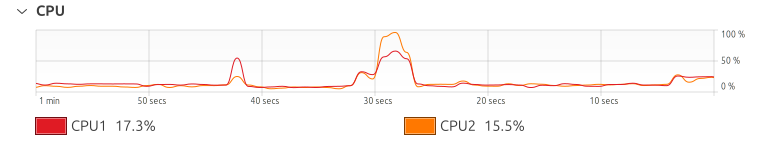
\includegraphics[width=0.8\linewidth]{thesis/23.png}
    \caption{CPU Usage after using Suricata}
    \label{fig:enter-label}
\end{figure}
\\ To assess whether Suricata was effective in mitigating the attack, the experiment was monitored using Wireshark on the victim machine. The following table summarizes the IPv4 traffic statistics during the attack window.
\begin{figure}[!htb]
    \centering
    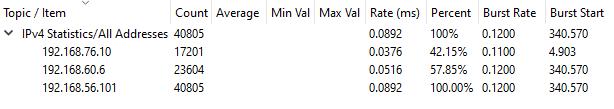
\includegraphics[width=0.8\linewidth]{thesis/scene2.png}
    \caption{Wireshark capture of scenario 2}
    \label{fig:enter-label}
\end{figure}
\begin{table}[!htb]
    \centering
    \scalebox{0.8}{
    \begin{tabular}{|m{6em}|c|c|c|c|c|c|c|c|}
    \hline
      Topic/Item & Count & Average & Min Val & Max Val & Rate(ms) & Percent & Burst Rate & Burst Start \\ 
      \hline
      IPv4 Statsistics/All addresses & 40805 &  &  & & 0.0892 & 100\% & 0.1200 & 340.570 \\
      \hline
      192.168.76.10 & 17201 & & & & 0.0376 & 42.15\% & 0.1100 & 4.903 \\
      \hline
      192.168.60.6 & 23604 & & & & 0.0516 & 57.85\% & 0.1200 & 340.570 \\
      \hline
      192.168.56.101 & 40805 & & & & 0.0892 & 100.00\% & 0.1200 & 340.570 \\
      \hline
    \end{tabular}}
    \caption{Wireshark statistics of scenario 2}
    \label{tab:my_label}
\end{table}
\\
Although Suricata was proactively specifying to drop incoming UDP, Wireshark established that very little packets were blocked on the victim. Traffic rates and burst rates reveal that there is a big number of UDP packets that the attack targeted on the victim machine.
\\
\begin{figure}[!htb]
    \centering
    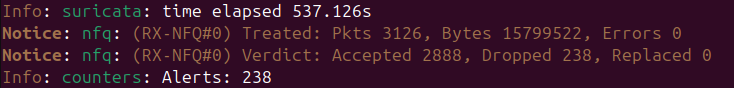
\includegraphics[width=0.8\linewidth]{thesis/report2.png}
    \caption{Suricata's report after the attack}
    \label{fig:enter-label}
\end{figure}
\\
As we can see, the traffic reports from wireshark and Suricata are different in terms of amount of packets. Under high pressure traffic, Suricata cannot handle very well, it only dropped a little amount compared to the number of packets that go through the network.
\subsection{Scenario 3: Reduced UDP Rates Attack with Suricata IPS Mode}
In this experiment, there will be some modifications to previous hping3 command. Instead of flooding the victim with UDP packets. We will reduce the UDP packets rate to the victim machine in order to observe Suricata working. In order to check how Suricata can behave with the acceptable traffic volume, the UDP flood was configured differently where it was set up to attack at low-rate. This time, every penetrating machine transmitted one packet every 200 milliseconds by the help of the following hping3 command.
\begin{lstlisting}[language=bash,caption={Modified ddos.sh}]
$ sudo hping3 --udp -d 120 --interval u200000 192.168.56.101
\end{lstlisting}
\\
Suricata was continued in IPS mode and set to drop all the UDP packets sent to the victim server (192.168.56.101). In this test Wireshark captured the following traffic statistics on the victim:
\begin{figure}[!htb]
    \centering
    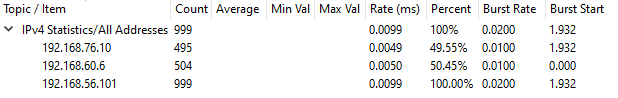
\includegraphics[width=0.8\linewidth]{thesis/s3Wireshark.png}
    \caption{Wireshark capture of scenario 3}
    \label{fig:enter-label}
\end{figure}
\begin{table}[!htb]
    \centering
    \scalebox{0.8}{
    \begin{tabular}{|m{6em}|c|c|c|c|c|c|c|c|}
    \hline
      Topic/Item & Count & Average & Min Val & Max Val & Rate(ms) & Percent & Burst Rate & Burst Start \\ 
      \hline
      IPv4 Statsistics/All addresses & 999 &  &  & & 0.0099 & 100\% & 0.0200 & 1.932 \\
      \hline
      192.168.76.10 & 495 & & & & 0.0049 & 49.55\% & 0.0100 & 1.932 \\
      \hline
      192.168.60.6 & 504 & & & & 0.0050 & 50.45\% & 0.0100 & 0.000 \\
      \hline
      192.168.56.101 & 999 & & & & 0.0099 & 100.00\% & 0.0200 & 1.932 \\
      \hline
    \end{tabular}}
    \caption{Wireshark statistics of scenario 3}
    \label{tab:my_label}
\end{table}
\\
These values confirm that the flood rate was much lower than in the high-speed test and are equivalent to 999 received packets on the victim. When Suricata IPS is turned off after the attack, it showed the following internal logs.
\pagebreak
\begin{figure}[!htb]
    \centering
    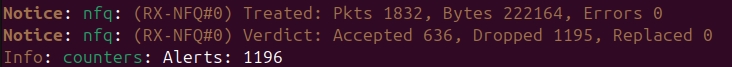
\includegraphics[width=0.8\linewidth]{thesis/s3Suricata.png}
    \caption{Suricata logs}
    \label{fig:enter-label}
\end{figure}
\\
We can clearly see that the system is under much less stress. CPU usage and network traffic are both significantly reduced.
\begin{figure}[!htb]
    \centering
    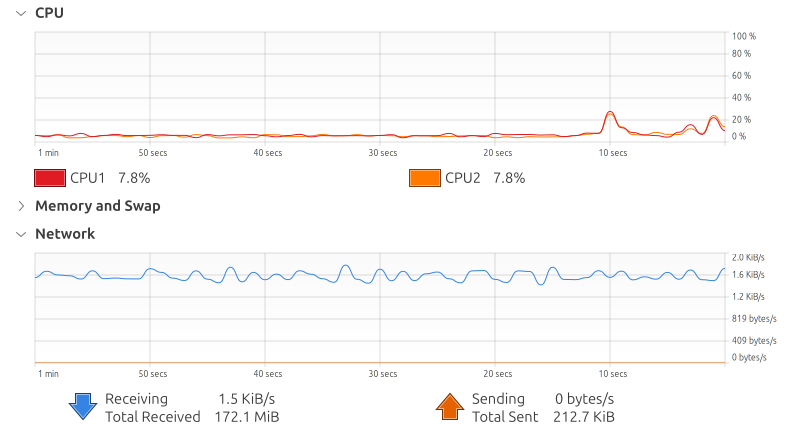
\includegraphics[width=0.8\linewidth]{thesis/s3Status.png}
    \caption{Victim resources usage during scenario 3}
    \label{fig:enter-label}
\end{figure}
\\
In this scenario, Suricata IPS performs considerably more effective than while under high-rate UDP flood. Approximately 65.25\% of attacker's bot UDP packets were successfully dropped (1195 dropped / 1832 total treated), the increase in drop rate is a strong indication that Suricata IPS can effectively counter UDP floods. Nevertheless, the success is defined by the frequency of incoming traffic and ability of the system to process the packets using NFQUEUE.
\\
\section{Comparative Results of UDP Flood Attack Scenarios}
The comparative analysis proves that Suricata may become an effective IPS in case it is properly set up and the network traffic does not overload. Still, its drawbacks when faced with high-speed attacks indirectly indicate the necessity of the use of the layer of defense. In practice, a need to combine the use of Suricata with hardware firewalls, upstream filtering, and rate-limiting policies could be of importance, with the purpose to achieve DDoS mitigation efficiently. The observation which is made with the help of Wireshark statistics and Suricata logs is one that leads to the verification of effectiveness of intrusion prevention in a case of simulated environments.
\begin{table}[!htb]
    \centering
    \scalebox{0.9}{
    \begin{tabular}{|c|c|c|c|c|}
    \hline
    Scenario  & Packets sent &  Packets received & Packets dropped & Suricata Effectiveness\\
    \hline
    Without IPS  & 48,082 &  48,082 & 0 & No protection \\
    \hline
    With IPS & 40,805 & 40,567 & 238 & Ineffective \\
    \hline
    Reduced rate with IPS & 1832 & 636 & 1195 & Effective (low-rate)\\
    \hline
    \end{tabular}}
    \caption{Summary Comparison Table}
    \label{tab:my_label}
\end{table}
\\
\section{Analysis of Suricata’s Limitations}
This finding clearly demonstrates that Suricata IPS failed to effectively counter the UDP flood because it was installed under the high traffic environment, so it needs the help of other tools such as firewall, window defender, etc. \cite{johnson2025suricata}. This behavior can be attributed to a few factors:
\begin{itemize}
\item NFQUEUE queue saturation \\
At high loads, the NFQUEUE performer in the Linux kernel can drop or bypass a subset of packets without inspecting it by Suricata.
\item Resource bottlenecks \\
User-space Suricata may be overpowered by a high-rate attack because it runs at an upper limit of processing resources available to a host.
\item Timing mismatch \\
Suricata can start considering the traffic slightly later than receiving the first packets and thus letting some goes through.

\end{itemize}
\section{Stealth Behavior of Botnet Agents}
\\
One notable observation during the UDP flood simulation was the stealth operation of the zombie machines. When the start\_attack.sh script is executed from the attacker’s main controller machine, the targeted zombie machines initiate packet transmission without displaying any immediate or visible output on their local terminals. This characteristic mimics a realistic botnet operation, where compromised hosts silently execute commands without user awareness, making detection by casual monitoring difficult \cite{rodrigues2025kali}.
\begin{figure}[!htb]
    \centering
    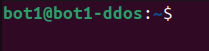
\includegraphics[width=0.3\linewidth]{thesis/bot1Stealth.png}
    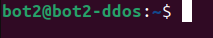
\includegraphics[width=0.4\linewidth]{thesis/bot2Stealth.png}
    \caption{Nothing changes on the zombie machines' terminals}
    \label{fig:enter-label}
\end{figure}
\\
An administrator or user who monitors the machine in real time, has no way of knowing malicious activity unless a further investigation is done (e.g. on the network monitor tools or system logs) because the bot machines do not print any output or logs to the terminal by default. The following is the output when hping3 command is conducted manually on zombie machines.
\begin{figure}[!htb]
    \centering
    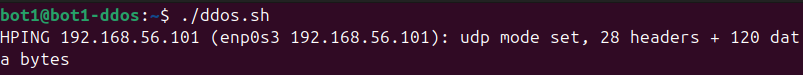
\includegraphics[width=0.8\linewidth]{thesis/ddosNoSsh.png}
    \caption{Output when ddos.sh is manually executed}
    \label{fig:enter-label}
\end{figure}
\\
The stealth attribute which underlines the role of host-based intrusion detection systems (HIDS) and network monitoring solutions. This attack does not create any foreground activity, therefore it cannot be happened but through passive monitoring. Rather, the security departments are forced to utilize Network Monitoring on Bot Machines or capturing of traffics through softwares like wireshark, etc.